% ============================================================================
%  RunTrack — Project Report (technology-focused, condensed edition)
%  Compile with pdfLaTeX on Overleaf (two passes for TOC/LOF/LOT).
% ============================================================================
\documentclass[12pt, a4paper]{report}

% ----------------------------- Packages -------------------------------------
\usepackage[T1]{fontenc}
\usepackage[utf8]{inputenc}
\usepackage{lmodern}
\usepackage[a4paper, top=2.6cm, bottom=2.6cm, left=2.8cm, right=2.2cm,
            headheight=15pt, headsep=18pt, footskip=30pt]{geometry}
\usepackage{setspace}
\usepackage{microtype}
\usepackage{fancyhdr}
\usepackage{titlesec}
\usepackage{graphicx}
\usepackage{booktabs}
\usepackage{tabularx}
\usepackage{array}
\usepackage{xcolor}
\usepackage{amsmath, amssymb}
\usepackage{enumitem}
\usepackage{float}
\usepackage[font=small, labelfont=bf, skip=6pt]{caption}
\usepackage{tikz}
\usetikzlibrary{arrows.meta, decorations.pathreplacing}
\usepackage{listings}
\usepackage[colorlinks=true, linkcolor=blue!55!black, urlcolor=blue!70!black,
            citecolor=blue!55!black, pdfauthor={RunTrack Project Team},
            pdftitle={RunTrack -- Project Report}]{hyperref}

% ----------------------------- Page style -----------------------------------
\onehalfspacing
\setlength{\parindent}{1.2cm}
\setlength{\parskip}{2pt}

\pagestyle{fancy}
\fancyhf{}
\fancyhead[L]{\small\itshape RunTrack}
\fancyhead[R]{\small\itshape Project Report}
\fancyfoot[C]{\small\thepage}
\renewcommand{\headrulewidth}{0.4pt}
\renewcommand{\footrulewidth}{0pt}

\titleformat{\chapter}[display]
  {\normalfont\bfseries\Huge}{\chaptertitlename\ \thechapter}{16pt}{\Huge}
\titleformat{\section}{\normalfont\Large\bfseries}{\thesection}{0.7em}{}
\titleformat{\subsection}{\normalfont\large\bfseries}{\thesubsection}{0.7em}{}
\titlespacing*{\chapter}{0pt}{-10pt}{28pt}
\titlespacing*{\section}{0pt}{16pt}{8pt}
\titlespacing*{\subsection}{0pt}{12pt}{6pt}

\setlist{itemsep=4pt, topsep=6pt, parsep=0pt}
\newcolumntype{C}{>{\centering\arraybackslash}X}
\newcolumntype{L}{>{\raggedright\arraybackslash}X}

% ----------------------------- Editable details -----------------------------
\newcommand{\institution}{[Your Institution Name]}
\newcommand{\department}{[Department of Computer Engineering]}
\newcommand{\university}{[University / Board Name]}
\newcommand{\courseTitle}{Cross Platform App Development (CPAD)}
\newcommand{\academicYear}{2025--2026}
\newcommand{\reportDate}{November 2026}
\newcommand{\guideName}{[Guide Name, Designation]}

% ----------------------------- Helper macros --------------------------------
\newcommand{\pkg}[1]{\texttt{#1}}
\newcommand{\code}[1]{\texttt{#1}}
\newcommand{\starchapter}[1]{%
  \chapter*{#1}%
  \markboth{#1}{#1}%
  \addcontentsline{toc}{chapter}{#1}}

% Screenshot placeholder cell
\newcommand{\shot}[3]{%
  \f\boxed{\parbox[c][3.6cm][c]{#1}{%
    \centering\textcolor{black!45}{\textbf{#2}}\\[3pt]
    \footnotesize\textcolor{black!40}{#3}}}}

% ----------------------------- Code listings --------------------------------
\lstdefinelanguage{TypeScript}{
  morekeywords={const,let,var,function,return,async,await,export,default,
    import,from,interface,type,extends,implements,new,class,if,else,for,while,
    switch,case,break,continue,typeof,instanceof,void,null,undefined,true,false,
    this,try,catch,finally,throw,public,private,readonly,static,as,of,in,delete,
    yield,enum,declare,namespace,keyof,satisfies,any,string,number,boolean,
    unknown,never},
  sensitive=true,
  morecomment=[l]{//},
  morecomment=[s]{/*}{*/},
  morestring=[b]"
}
\lstset{
  language=TypeScript,
  basicstyle=\ttfamily\footnotesize,
  keywordstyle=\color{blue!65!black},
  commentstyle=\color{green!45!black},
  stringstyle=\color{orange!75!black},
  numbers=left,
  numberstyle=\tiny\color{black!45},
  numbersep=8pt,
  frame=single,
  framerule=0.4pt,
  rulecolor=\color{black!35},
  breaklines=true,
  showstringspaces=false,
  tabsize=2,
  xleftmargin=1.6em,
  framexleftmargin=1.4em,
  aboveskip=10pt,
  belowskip=10pt,
  columns=flexible
}

% ----------------------------- TikZ styles ----------------------------------
\tikzset{
  entity/.style={rectangle, draw=black!70, fill=blue!6, inner sep=6pt,
                 font=\footnotesize, align=left},
  rel/.style={diamond, draw=black!70, fill=yellow!20, inner sep=2pt,
              font=\footnotesize, align=center},
  lbl/.style={font=\scriptsize, fill=white, inner sep=1.5pt}
}

% ============================================================================
%                              FRONT MATTER
% ============================================================================
\begin{document}
\pagenumbering{roman}

% ----------------------------- Title page -----------------------------------
\begin{titlepage}
\begin{center}
\vspace*{0.5cm}
{\rule{\textwidth}{1.2pt}}\\[0.4cm]
{\large\bfseries \institution}\\[0.2cm]
{\large\bfseries \department}\\[0.1cm]
{\normalsize Affiliated to \university}\\[0.5cm]
{\rule{\textwidth}{0.6pt}}\\[1.8cm]

{\LARGE\bfseries RUNTRACK}\\[0.5cm]
{\Large\bfseries A Strava-Style GPS Fitness Activity Tracker}\\[1.2cm]

{\large A Project Report}\\[0.3cm]
{\normalsize Submitted in partial fulfilment of the requirements for the award
of the degree}\\[0.15cm]
{\normalsize in Bachelor of Technology / Diploma}\\[0.15cm]
{\normalsize in Computer Engineering / Computer Science}\\[0.8cm]

{\normalsize Under the guidance of}\\[0.3cm]
{\large\bfseries \guideName}\\[1.5cm]

\vfill

{\normalsize \textbf{Course:} \courseTitle \hfill
             \textbf{Academic Year:} \academicYear}\\[0.4cm]
{\normalsize \textbf{Submitted by:}}\\[0.3cm]
\begin{tabular}{@{}ccl@{}}
  \textbf{S.\,No.} & \textbf{Name of Student} & \textbf{Roll No.}\\[2pt]
  1 & [Student Name 1] & [Roll No.\ 1]\\
  2 & [Student Name 2] & [Roll No.\ 2]\\
  3 & [Student Name 3] & [Roll No.\ 3]\\
\end{tabular}\\[1.0cm]
{\normalsize \reportDate}\\[0.5cm]
{\rule{\textwidth}{1.2pt}}
\end{center}
\end{titlepage}

% ------------- Certificate, Declaration, Acknowledgement (one page) ---------
\starchapter{Certificate, Declaration and Acknowledgement}

\section*{Certificate}
\noindent
This is to certify that the project report entitled \textbf{``RunTrack ---
A Strava-Style GPS Fitness Activity Tracker''} is a bonafide record of work
carried out by \textbf{[Student Names / Roll Numbers]} under our supervision
during the academic year \textbf{\academicYear} in partial fulfilment of the
requirements for the degree in \textbf{[Degree Name]}.

\vspace{1.2cm}
\noindent
\begin{tabularx}{\textwidth}{@{}X X@{}}
\textbf{Internal Guide} & \textbf{Head of Department}\\[1.4cm]
\underline{\hspace{5.5cm}} & \underline{\hspace{5.5cm}}\\[0.2cm]
\guideName & [HOD Name, Designation]
\end{tabularx}

\vspace{1.4cm}
\section*{Declaration}
\noindent
We declare that this report is our own original work; the results presented
have not been submitted, in whole or in part, for any other degree or
certificate of this or any other institution. All sources of information
used have been duly acknowledged.

\vspace{1.6cm}
\noindent
\begin{tabularx}{\textwidth}{@{}X X X@{}}
\underline{\hspace{4.5cm}} & \underline{\hspace{4.5cm}} &
\underline{\hspace{4.5cm}}\\[0.2cm]
[Student 1] & [Student 2] & [Student 3]
\end{tabularx}

\vspace{0.8cm}
\section*{Acknowledgement}
\noindent
We thank our guide \guideName, the Head of the Department
\department, and the faculty of \courseTitle for their guidance, facilities,
and encouragement, and our families for their support.

% ----------------------------- Abstract -------------------------------------
\starchapter{Abstract}
\vspace{0.4cm}
\noindent
\textbf{Keywords:} React Native, Expo, TypeScript, Firebase, Cloud Firestore,
GPS tracking, offline-first, SQLite, Zustand, Vitest.

\vspace{0.5cm}
\noindent
RunTrack is a cross-platform GPS fitness tracker built with \textbf{React
Native (Expo SDK 58)} and backed by \textbf{Firebase}. It records runs,
cycles, and walks from the device GPS, computes distance (Haversine),
pause-aware duration, pace, and calories, and stores every activity in
\textbf{Cloud Firestore} through owner-only security rules. The system is
\textbf{offline-first}: saves are written to a local \textbf{SQLite} queue
first and pushed to the cloud by a synchronisation worker whenever
connectivity returns. Value-adding features include an AI workout-recap
pipeline hosted in a \textbf{Cloud Function} (so no API key ships in the
app bundle), badges and streaks, per-kilometre \textbf{expo-speech} voice
coaching, and a route heatmap.

\vspace{0.4cm}
\noindent
The report focuses on the \textbf{technology stack}: why each technology was
chosen over its alternatives, how the platform APIs are configured, and how
the layers fit together. The implementation is written in strict TypeScript
and verified by \textbf{593 unit tests across 25 files}, ESLint, type
checking, Expo Doctor (20/20), and a production Hermes bundle export.

% ----------------------------- TOC / LOF / LOT ------------------------------
\cleardoublepage
\tableofcontents
\cleardoublepage
\listoffigures
\cleardoublepage
\listoftables

% ============================================================================
\pagenumbering{arabic}
\setcounter{page}{1}

\chapter{Introduction}
\markboth{Chapter 1: Introduction}{Chapter 1: Introduction}

\section{Background}
Smartphones with GPS receivers have made personal fitness tracking everyday
practice, and applications such as Strava and Nike Run Club have shown the
familiar pattern: record a workout, draw it on a map, compute statistics, and
review history. RunTrack rebuilds that pattern as a college mini project in
\courseTitle, deliberately using a \textbf{single frontend framework}
(React Native via Expo) and a \textbf{genuine cloud backend} (Firebase), so
that the complete path from a GPS fix on the device to a document in a cloud
database is implemented, secured, and tested by the student team.

\section{Objectives}
\begin{enumerate}[leftmargin=1.2cm]
  \item Record outdoor activities (run/cycle/watch) with GPS, a live map
        polyline, and live statistics.
  \item Compute distance, duration, pace, and calories with testable pure
        functions.
  \item Persist activities in an integrated backend (Firebase Authentication
        + Cloud Firestore) with owner-only security rules.
  \item Keep recording and saving fully functional \textbf{without
        connectivity} through a local SQLite queue and automatic sync.
  \item Add AI workout recaps, badges/streaks, voice coaching, and a route
        heatmap without blocking the core loop.
  \item Verify the system with unit tests, static analysis, and documented
        manual QA.
\end{enumerate}

\section{Scope and Limitations}
\textbf{In scope:} authentication and session persistence; foreground GPS
tracking with pause/resume and confirmation-protected stop; statistics;
local-first save with cloud sync; History and Activity Detail screens; AI
recap design; badges, streaks, and profile aggregates; voice coaching; route
heatmap; themed UI with loading, empty, and error states; security rules;
unit tests.

\textbf{Out of scope:} elevation/altitude, social features (kudos, friends,
leaderboards), wearable/health-app integration, and a km/mi unit toggle.

\textbf{Known limitations:} tracking is foreground-only (backgrounding
auto-pauses; the screen stays awake during a run); an unsaved live session
lives in memory and is lost on process death (a \emph{completed} save is
durable in SQLite); and device-level acceptance testing with real Firebase
credentials remains pending, as recorded in the project QA checklists.

\section{Report Organisation}
Chapter~2 states the requirements. Chapter~3 gives the system overview and
design essentials. Chapter~4 --- the core of this report --- studies the
\textbf{technology stack} in depth. Chapter~5 presents the implementation of
the key modules, Chapter~6 the testing and quality assurance,
Chapter~7 the results, and Chapter~8 the conclusion and future scope.

% ============================================================================
\chapter{Requirements Analysis}
\markboth{Chapter 2: Requirements Analysis}{Chapter 2: Requirements Analysis}

\section{Functional Requirements}
\begin{table}[H]
\centering
\caption{Functional requirements}
\label{tab:fr}
\small
\begin{tabularx}{\textwidth}{@{}l L@{}}
\toprule
\textbf{ID} & \textbf{Requirement} \\
\midrule
FR-01 & \textbf{Registration:} account with name, e-mail, password
        ($\geq$ 6 characters) plus a matching profile document. \\
FR-02 & \textbf{Login / Logout:} e-mail/password sign-in, session persisted
        across restarts, logout from Profile. \\
FR-03 & \textbf{Activity type:} select Run, Cycle, or Walk before recording;
        the choice flows through tracking, saving, and history. \\
FR-04 & \textbf{GPS tracking:} request precise foreground permission,
        subscribe to fixes, draw the live route as a map polyline. \\
FR-05 & \textbf{Live statistics:} elapsed time, distance, and current pace
        while recording. \\
FR-06 & \textbf{Pause / Resume:} freeze the timer and distance; resume starts
        a new route segment. \\
FR-07 & \textbf{Stop with confirmation:} an explicit dialog prevents
        accidental end-of-workout. \\
FR-08 & \textbf{Statistics:} Haversine distance, duration minus pauses,
        average pace (min:sec/km), weight-based calorie estimate. \\
FR-09 & \textbf{Activity review:} summary screen with route and stats;
        Save or Discard before any database write. \\
FR-10 & \textbf{Cloud persistence:} saving writes an owner-attributed
        activity to Cloud Firestore. \\
FR-11 & \textbf{Offline save:} every save first lands in a local SQLite
        queue, so no completed activity is ever lost. \\
FR-12 & \textbf{Automatic sync:} queued rows upload when connectivity
        returns (retry with backoff) with a pending-sync banner. \\
FR-13 & \textbf{History:} latest 50 activities, newest first, with type,
        date, distance, duration, and pace. \\
FR-14 & \textbf{Activity Detail:} stored statistics plus an interactive
        route map. \\
FR-15 & \textbf{AI recap:} short generated summary via a server-side Cloud
        Function; failure never blocks saving. \\
FR-16 & \textbf{Gamification:} badges and streaks re-evaluated after each
        save, displayed on Profile. \\
FR-17 & \textbf{Voice coaching:} per-kilometre text-to-speech announcements
        with a persisted mute preference. \\
FR-18 & \textbf{Heatmap:} all past routes overlaid on one map. \\
\bottomrule
\end{tabularx}
\end{table}

\section{Non-Functional Requirements}
\begin{table}[H]
\centering
\caption{Non-functional requirements}
\label{tab:nfr}
\small
\begin{tabularx}{\textwidth}{@{}l L@{}}
\toprule
\textbf{Category} & \textbf{Requirement} \\
\midrule
Reliability & No completed activity may be lost; local write precedes every
  network attempt. \\
Performance & Live UI follows the GPS cadence without blocking; History is
  capped at 50 rows; SQLite WAL keeps saves from blocking reads. \\
Security & Owner-only access enforced by Firestore rules (default-deny);
  no server secret in the mobile bundle. \\
Offline & Recording and saving must work with no connectivity. \\
Usability & One theme (design tokens), loading indicators for every async
  operation, non-blocking toasts, confirm dialogs only for destructive
  actions. \\
Maintainability & Strict TypeScript, ESLint, layered architecture, pure
  utility functions, unit tests for all business logic. \\
Portability & Expo managed workflow (no hand-written native projects);
  Android, iOS, and a web fallback. \\
Data integrity & Activities are create-only; the only mutable field is the
  owner-only AI recap; sync retries are idempotent. \\
\bottomrule
\end{tabularx}
\end{table}

% ============================================================================
\chapter{System Overview and Design}
\markboth{Chapter 3: System Overview and Design}
          {Chapter 3: System Overview and Design}

\section{Layered Architecture}
Screens never talk to Firebase or the GPS directly: they call services,
services call the repository layer, and only that layer touches the backend.
Figure~\ref{fig:arch} shows the layers.

\begin{figure}[H]
\centering
\resizebox{\textwidth}{!}{%
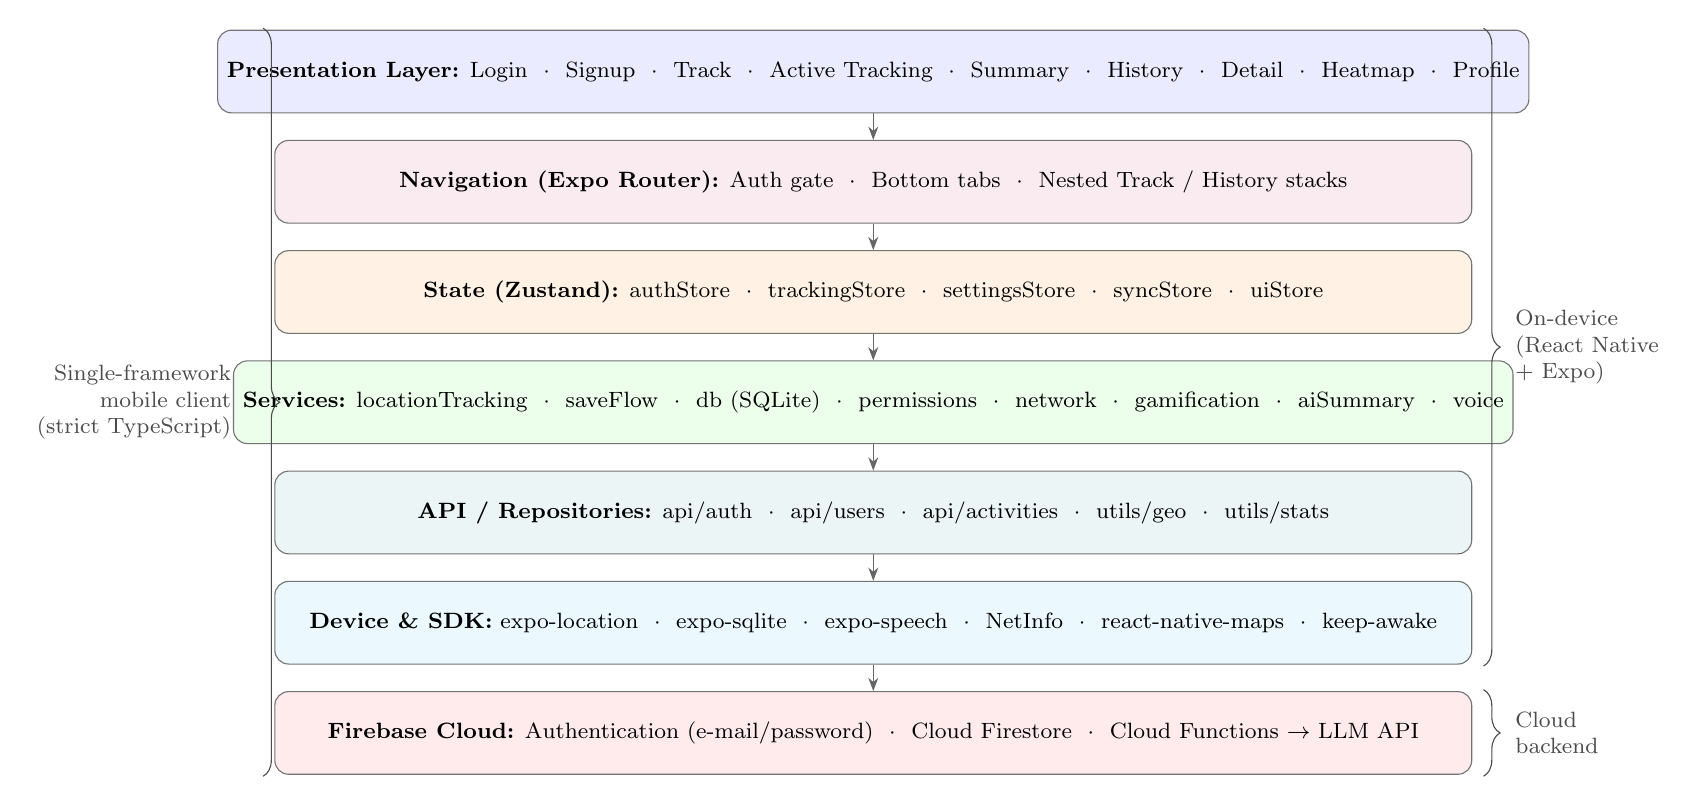
\begin{tikzpicture}[font=\footnotesize]
  \def\roww{15.2cm}
  \node[rectangle, rounded corners=5pt, draw=black!55, fill=blue!8,
        minimum width=\roww, minimum height=1.05cm, align=center] (r1) at (0,0)
        {\textbf{Presentation Layer:} Login \ $\cdot$ \ Signup \ $\cdot$ \ Track
         \ $\cdot$ \ Active Tracking \ $\cdot$ \ Summary \ $\cdot$ \ History
         \ $\cdot$ \ Detail \ $\cdot$ \ Heatmap \ $\cdot$ \ Profile};
  \node[rectangle, rounded corners=5pt, draw=black!55, fill=purple!8,
        minimum width=\roww, minimum height=1.05cm, align=center] (r2) at (0,-1.4)
        {\textbf{Navigation (Expo Router):} Auth gate \ $\cdot$ \ Bottom tabs
         \ $\cdot$ \ Nested Track / History stacks};
  \node[rectangle, rounded corners=5pt, draw=black!55, fill=orange!10,
        minimum width=\roww, minimum height=1.05cm, align=center] (r3) at (0,-2.8)
        {\textbf{State (Zustand):} authStore \ $\cdot$ \ trackingStore
         \ $\cdot$ \ settingsStore \ $\cdot$ \ syncStore \ $\cdot$ \ uiStore};
  \node[rectangle, rounded corners=5pt, draw=black!55, fill=green!8,
        minimum width=\roww, minimum height=1.05cm, align=center] (r4) at (0,-4.2)
        {\textbf{Services:} locationTracking \ $\cdot$ \ saveFlow \ $\cdot$ \ db
         (SQLite) \ $\cdot$ \ permissions \ $\cdot$ \ network \ $\cdot$ \
         gamification \ $\cdot$ \ aiSummary \ $\cdot$ \ voice};
  \node[rectangle, rounded corners=5pt, draw=black!55, fill=teal!8,
        minimum width=\roww, minimum height=1.05cm, align=center] (r5) at (0,-5.6)
        {\textbf{API / Repositories:} api/auth \ $\cdot$ \ api/users \ $\cdot$ \
         api/activities \ $\cdot$ \ utils/geo \ $\cdot$ \ utils/stats};
  \node[rectangle, rounded corners=5pt, draw=black!55, fill=cyan!8,
        minimum width=\roww, minimum height=1.05cm, align=center] (r6) at (0,-7.0)
        {\textbf{Device \& SDK:} expo-location \ $\cdot$ \ expo-sqlite \ $\cdot$ \
         expo-speech \ $\cdot$ \ NetInfo \ $\cdot$ \ react-native-maps
         \ $\cdot$ \ keep-awake};
  \node[rectangle, rounded corners=5pt, draw=black!55, fill=red!8,
        minimum width=\roww, minimum height=1.05cm, align=center] (r7) at (0,-8.4)
        {\textbf{Firebase Cloud:} Authentication (e-mail/password) \ $\cdot$ \
         Cloud Firestore \ $\cdot$ \ Cloud Functions $\rightarrow$ LLM API};

  \foreach \a/\b in {r1/r2, r2/r3, r3/r4, r4/r5, r5/r6, r6/r7} {
    \draw[-{Stealth}, black!60] (\a.south) -- (\b.north);
  }

  \draw[decorate, decoration={brace, amplitude=6pt}, black!70]
        (7.75,0.55) -- (7.75,-7.55)
        node[midway, right=8pt, font=\footnotesize, align=left]
        {On-device\\(React Native\\+ Expo)};
  \draw[decorate, decoration={brace, amplitude=6pt}, black!70]
        (7.75,-7.85) -- (7.75,-8.95)
        node[midway, right=8pt, font=\footnotesize, align=left]
        {Cloud\\backend};
  \draw[decorate, decoration={brace, amplitude=6pt}, black!70]
        (-7.75,0.55) -- (-7.75,-8.95)
        node[midway, left=8pt, font=\footnotesize, align=right]
        {Single-framework\\mobile client\\(strict TypeScript)};
\end{tikzpicture}}
\caption{Layered system architecture of RunTrack}
\label{fig:arch}
\end{figure}

The key architectural rules are: screens only orchestrate state; a single
service owns the GPS watch and the one keep-awake lock; distance, pace, and
formatting are pure functions (which is what makes the test suite fast); and
optional features (AI recap, gamification) can never turn a successful save
into a failure.

\section{Navigation}
\pkg{expo-router} maps files under \code{src/app/} to routes
(Figure~\ref{fig:nav}). The root layout owns the auth gate --- signed-out
users are redirected to Login --- plus the navigation theme, toast host, and
tracking lifecycle cleanup. Route parameters are typed, so a link such as
\code{/history/[activityId]} is validated at compile time.

\begin{figure}[H]
\centering
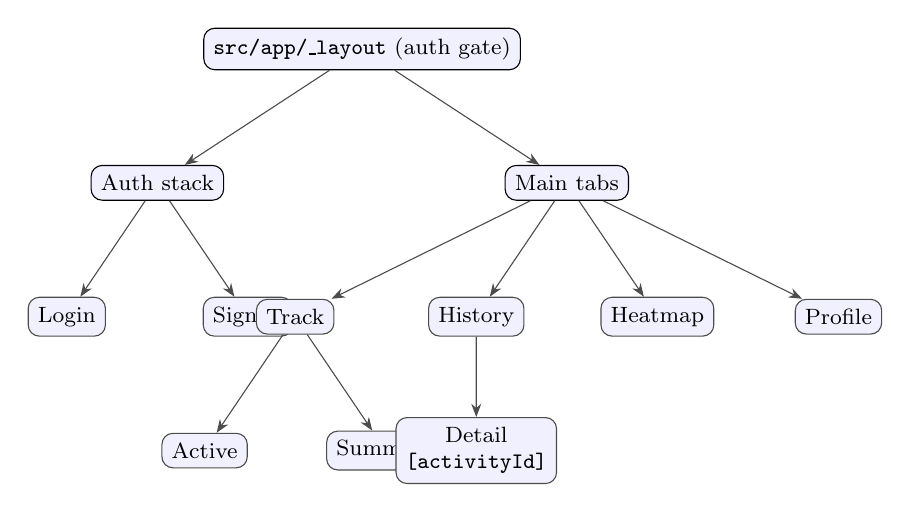
\begin{tikzpicture}[
  level 1/.style={sibling distance=5.2cm, level distance=1.7cm},
  level 2/.style={sibling distance=2.3cm, level distance=1.7cm},
  every node/.style={draw, rounded corners, fill=blue!6, font=\footnotesize,
                     align=center, inner sep=3.5pt},
  edge from parent/.style={draw, -{Stealth}, black!70}
]
\node {\texttt{src/app/\_layout} (auth gate)}
  child {node {Auth stack}
    child {node {Login}}
    child {node {Signup}}
  }
  child {node {Main tabs}
    child {node {Track}
      child {node {Active}}
      child {node {Summary}}
    }
    child {node {History}
      child {node {Detail \\ \texttt{[activityId]}}}
    }
    child {node {Heatmap}}
    child {node {Profile}}
  };
\end{tikzpicture}
\caption{Navigation structure (Expo Router file-based routes)}
\label{fig:nav}
\end{figure}

\section{Data Model}
The database is document-oriented (Cloud Firestore) plus one local SQLite
table. Figure~\ref{fig:er} shows the entity-relationship view.

\begin{figure}[H]
\centering
\begin{tikzpicture}[font=\footnotesize]
  \node[entity] (users) at (0,5.0) {
    \textbf{users} \hfill \textit{1}\\[3pt]
    \underline{uid} : string \ \ (PK)\\
    name : string\\
    email : string\\
    weightKg : number \ \ (default 70)\\
    createdAt : timestamp\\
    totalDistanceKm : number\\
    totalActivities : number\\
    currentStreak : number\\
    longestStreak : number\\
    lastActivityDate : string\\
    badges : string[]};

  \node[entity] (acts) at (-4.9,-2.2) {
    \textbf{activities} \hfill \textit{N}\\[3pt]
    \underline{activityId} : string \ \ (PK)\\
    userId : string \ \ (FK, indexed)\\
    type : ``run'' $\vert$ ``cycle'' $\vert$ ``walk''\\
    startTime : timestamp\\
    endTime : timestamp\\
    durationSec : number\\
    distanceKm : number\\
    avgPaceSecPerKm : number\\
    caloriesEstimate : number\\
    route : \{lat, lng, timestamp\}[]\\
    aiSummary : string \ \ (optional)\\
    createdAt : timestamp};

  \node[entity] (heat) at (5.8,2.0) {
    \textbf{users/\{uid\}/heatmapPoints} \hfill \textit{N}\\[3pt]
    \underline{pointId} : string \ \ (PK)\\
    userId : string \ \ (FK)\\
    day : string \ \ (YYYY-MM-DD)\\
    distanceKm : number};

  \node[entity] (pend) at (1.7,-6.2) {
    \textbf{pending\_activities} \ \ \textit{(local SQLite)}\\[3pt]
    \underline{localId} : string \ \ (PK)\\
    firestoreId : string \ \ (nullable)\\
    userId, type, startTime, endTime : as activities\\
    distanceKm, durationSec, pace, calories : as activities\\
    route : JSON text\\
    synced : boolean \ \ (0 / 1)\\
    retryCount, lastAttempt : integer\\
    createdAt : integer \ \ (epoch ms)};

  \node[rel] (r1) at (-2.45,1.6) {records};
  \node[rel] (r2) at (2.8,3.5) {generates};

  \draw[black!70] (users.south) -- (r1);
  \draw[black!70] (r1) -- (acts.north east);
  \node[font=\footnotesize] at (-1.0,2.6) {1};
  \node[font=\footnotesize] at (-3.6,0.7) {N};

  \draw[black!70] (users.east) -- (r2);
  \draw[black!70] (r2) -- (heat.west);
  \node[font=\footnotesize] at (2.1,4.4) {1};
  \node[font=\footnotesize] at (3.6,2.6) {N};

  \draw[black!60, dashed] (acts.south east) -- (pend.west)
        node[lbl, midway, above, sloped]
        {mirrors until synced};
\end{tikzpicture}
\caption{Entity--relationship diagram of the RunTrack data model}
\label{fig:er}
\end{figure}

A composite index on (\code{userId}, \code{startTime} descending) serves the
History query. Activities are \emph{create-only}: the single permitted
mutation is the owner-only \code{aiSummary} update, which keeps workout
history immutable.

% ============================================================================
\chapter{Technology Study}
\markboth{Chapter 4: Technology Study}{Chapter 4: Technology Study}

This chapter is the core of the report: it explains \emph{why} each
technology in RunTrack was chosen, how it is configured on this project, and
what alternatives were rejected.

\section{Selection Criteria}
The stack had to satisfy four constraints simultaneously:

\begin{enumerate}[leftmargin=1.2cm]
  \item \textbf{Single framework} --- one codebase for Android, iOS, and web.
  \item \textbf{Integrated backend + database} --- a real cloud service, not
        local-only storage.
  \item \textbf{Device capability access} --- GPS, maps, local database, and
        text-to-speech must all be reachable without writing native code.
  \item \textbf{Lab-project timeframe} --- managed workflows and minimal
        ceremony, so effort goes into features rather than tooling.
\end{enumerate}

\section{React Native with Expo (Managed Workflow)}
\textbf{React Native} renders native mobile UI from JavaScript/TypeScript
components, giving near-native performance with one codebase. \textbf{Expo}
adds a managed workflow around it: a single CLI configures native modules,
permissions, and cloud builds, eliminating hand-maintained Xcode and Android
Studio projects.

RunTrack uses \textbf{Expo SDK 58} (React Native 0.88.1, React 19.3) and
relies on three platform mechanisms:

\begin{itemize}[leftmargin=1.2cm]
  \item \textbf{Continuous Native Generation (CNG):} the \code{ios/} and
        \code{android/} projects are generated from \code{app.json} and
        config plugins on every build. They are never edited by hand, which
        removes an entire class of ``works on my machine'' drift.
  \item \textbf{Config plugins:} native behaviour is declared
        declaratively in \code{app.json} --- for example the
        \pkg{expo-location} plugin carries the permission strings
        (``RunTrack uses precise location to record your route while the app
        is open''), background location is explicitly disabled, and the
        \pkg{react-native-maps} plugin receives the Google Maps API keys.
  \item \textbf{Hermes engine:} the JavaScript engine compiled ahead-of-time
        into the binary improves start-up time and memory use; the production
        bundle is exported as a Hermes bundle as part of verification.
\end{itemize}

\noindent \textbf{Alternatives rejected:} bare React Native (rejected ---
native project maintenance overhead), Flutter (rejected --- the course
mandates React Native), and Ionic (rejected --- web-view rendering is a poor
fit for GPS/maps-heavy apps).

\section{TypeScript (Strict Mode)}
The whole codebase is \textbf{strict TypeScript} v6.0. Types document the
domain at compile time --- the activity shape, the \code{SaveOutcome} of a
save, the Zustand store contracts --- and the navigation's typed-routes
experiment validates every \code{router.push} href against the actual route
tree. \code{tsc --noEmit} is part of the project's definition of done, so
whole classes of runtime errors are eliminated before tests run.

\section{Expo Router (File-Based Navigation)}
\pkg{expo-router} is chosen over hand-wired React Navigation because routes
are simply files: \code{src/app/(auth)/login.tsx} \emph{is} the Login route.
Layout files compose navigators --- a root \code{\_layout.tsx} for the auth
gate, \code{(tabs)/\_layout.tsx} for the four-tab bar, and nested
\code{Stack} layouts inside Track and History. Typed routes generated by
\code{expo export} make an invalid deep link a compile error rather than a
runtime surprise.

\section{Firebase (Backend as a Service)}
Firebase satisfies the ``genuine integrated backend'' requirement with four
services, all consumed through the \textbf{Firebase JavaScript SDK v13.3}.

\subsection{Why the JS SDK instead of React Native Firebase}
\begin{table}[H]
\centering
\caption{Firebase client SDK options}
\label{tab:sdk}
\small
\begin{tabularx}{\textwidth}{@{}l L L@{}}
\toprule
 & \textbf{Firebase JS SDK} & \textbf{React Native Firebase} \\
\midrule
Platform support & Android, iOS, \textbf{and web} from one API & Android \&
  iOS only \\
Setup & Pure JS; no native config files & Requires native modules,
  \code{google-services.json}, re-builds \\
Session persistence & AsyncStorage via
  \code{getReactNativePersistence} & Built-in \\
Fit for this project & \textbf{Chosen} --- matches CNG and the web target &
  Rejected --- native config overhead \\
\bottomrule
\end{tabularx}
\end{table}

\subsection{Authentication}
E-mail/password sign-in with a minimum password length of six characters.
Session persistence uses AsyncStorage through
\code{getReactNativePersistence}; Firebase 13.3 exposes that symbol only via
the \code{react-native} runtime condition and omits it from the types
barrel, so a small typed module augmentation in \code{src/api/firebase.ts}
keeps strict mode intact. Session bootstrap is idempotent and guarded by an
8-second safety timer so a broken persistence layer can never hang the auth
gate.

\subsection{Cloud Firestore}
The primary database holds three collections: \code{users}, \code{activities}
(with the composite index mentioned in Section~3.3), and the
\code{heatmapPoints} sub-collection. Repository modules
(\code{api/users.ts}, \code{api/activities.ts}) are the only code that talks
to Firestore; they validate writes, whitelist fields, normalise remote
values, and convert Firestore \code{Timestamp} objects to epoch milliseconds
at the boundary, so screens never see SDK-specific types.

\subsection{Cloud Functions}
A single HTTPS callable function, \code{generateWorkoutSummary}, hosts the
AI recap. Keeping it server-side means the language-model API key is a
\emph{server secret} set with \code{firebase functions:secrets:set} and is
never part of the mobile bundle --- a hard security requirement, since any
value shipped to a device must be treated as public.

\subsection{Security rules}
Security lives in the backend, not the UI (full rules live in the project
repository, \code{firestore.rules}):

\begin{itemize}[leftmargin=1.2cm]
  \item \code{users/\{uid\}} and its \code{heatmapPoints} sub-collection:
        read/write only for the matching authenticated UID.
  \item \code{activities}: \textbf{create} only for documents attributed to
        oneself (this stops forging another user's history), \textbf{read}
        owner-only, \textbf{update} owner-only restricted to exactly the
        \code{aiSummary} key, \textbf{delete} never.
  \item A catch-all match \code{allow read, write: if false} --- the default
        is deny.
\end{itemize}

\subsection{Configuration hygiene}
Committed files contain only \code{PASTE\_...} placeholders; real Firebase
values live in the git-ignored \code{firebase.local.json}, merged at build
time by \code{app.config.js}. A guard (\code{assertFirebaseConfigured()})
rejects repository operations \emph{before} any Firestore request when
configuration is incomplete, so an unconfigured build fails honestly instead
of fabricating persistence. Client identifiers (Firebase config, Maps keys)
are distributed with every app by definition; they are protected by API
restrictions and security rules, not by secrecy.

\section{Zustand (State Management)}
Global state is held in five small \pkg{zustand} stores: \code{authStore}
(current user, bootstrap status), \code{trackingStore} (live session and the
frozen review snapshot), \code{settingsStore} (voice preference),
\code{syncStore} (pending-sync count), and \code{uiStore} (toast queue).

\begin{table}[H]
\centering
\caption{State-management options}
\label{tab:state}
\small
\begin{tabularx}{\textwidth}{@{}l L L@{}}
\toprule
 & \textbf{Zustand} & \textbf{Redux Toolkit} \\
\midrule
Boilerplate & Minimal (one hook + slices) & Action/reducer/thunk ceremony \\
Subscription & Selector-based; re-renders only changed slices & Requires
  memoised selectors or hooks \\
Bundle \& learning curve & Very small, trivial API & Larger, team convention
  needed \\
Fit & \textbf{Chosen} --- five simple stores, short timeline &
  Rejected --- overkill at this scope \\
\bottomrule
\end{tabularx}
\end{table}

\noindent React Query was also considered and rejected: History and Detail
need only focus-scoped subscriptions, not a caching layer.

\section{Offline-First Storage: expo-sqlite + NetInfo}
Offline recording is a headline requirement, so the persistence choice matters.

\begin{table}[H]
\centering
\caption{Local storage options}
\label{tab:localdb}
\small
\begin{tabularx}{\textwidth}{@{}l L L@{}}
\toprule
 & \textbf{expo-sqlite} & \textbf{AsyncStorage} \\
\midrule
Model & Relational tables, indexed queries & Single JSON blob per key \\
Concurrency & WAL journal mode: fast writes alongside open reads & Whole-blob
  read/rewrite \\
Migrations & \code{PRAGMA user\_version} ordered migrations & Manual version
  field \\
Fit & \textbf{Chosen} --- a queryable queue with \code{WHERE synced = 0}
  & Rejected --- fragile for structured queues \\
\bottomrule
\end{tabularx}
\end{table}

\noindent The queue table \code{pending\_activities} stores every completed
save with a \code{synced} flag, a \code{firestoreId} (so retries are
idempotent), and \code{retryCount}/\code{lastAttempt} for backoff. WAL mode
keeps the save-time insert fast even while History is reading. The
\code{@react-native-community/netinfo} library reports connectivity; the
save path treats only an \emph{explicit} offline signal as offline, so a
transient network guess can never lose an activity. Synced rows older than
30 days are purged so the table cannot grow without bound.

\section{Maps and Location}
\pkg{react-native-maps} provides the map, polyline, markers, and fitted
route cameras. On native platforms it renders Google Maps through API keys
supplied by the \code{react-native-maps} config plugin (separate restricted
keys for Android and iOS; plugin changes require a rebuilt binary, not an OTA
update). On web, where the plugin's keys do not apply, the component falls
back to an informational map so the UI stays functional.

\pkg{expo-location} owns positioning and permissions:

\begin{itemize}[leftmargin=1.2cm]
  \item Watch configuration: \code{Accuracy.Highest},
        \code{timeInterval: 2000} (an Android minimum interval, not a
        cross-platform promise of a fix every two seconds), and
        \code{distanceInterval: 5}.
  \item Only \emph{foreground} permission is requested; background location
        is deliberately disabled in the plugin config, documenting the
        foreground-only scope.
  \item \pkg{expo-keep-awake} holds a single tagged wake lock while
        recording so the screen never sleeps mid-run.
\end{itemize}

\noindent The GPS engine (Section~5.2) filters every fix --- accuracy worse
than 20\,m, stale or out-of-order timestamps, and implied speeds above
28\,m/s (teleport rejection) are discarded --- and accumulates distance
\emph{within segments} so a pause never draws a straight gap line across the
map.

\section{Text-to-Speech: expo-speech}
\pkg{expo-speech} exposes the platform speech engines with no permission
required. The coaching module announces every completed kilometre, calls
\code{Speech.stop()} before each \code{Speech.speak()} so utterances never
overlap, queues at most one announcement at a time, and persists the mute
preference in \code{settingsStore}.

\section{Testing Toolchain}
\begin{itemize}[leftmargin=1.2cm]
  \item \textbf{Vitest v5} --- runs the suite with mocked native and Firebase
        modules; the full suite completes in about three seconds.
  \item \textbf{ESLint 9} with \code{eslint-config-expo} --- style and
        correctness lint (\code{npx expo lint}).
  \item \textbf{Expo Doctor} --- dependency and config health
        (\code{npx expo-doctor}, 20/20).
  \item \textbf{Hermes export} --- proves the production bundle builds
        (\code{npx expo export --platform android}).
\end{itemize}

\noindent Mocking strategy: \pkg{expo-location}, \pkg{expo-sqlite}, maps, and
the Firebase SDK are replaced with controllable fakes, so tests exercise the
\emph{logic} (filtering, segmentation, save pipeline, migrations, stores)
deterministically on any machine. What mocks cannot prove --- real GPS,
native rendering, deployed rules --- is covered by manual QA checklists
(Chapter~6).

\section{Alternatives Considered --- Summary}
\begin{table}[H]
\centering
\caption{Technology decisions and rejected alternatives}
\label{tab:alt}
\small
\begin{tabularx}{\textwidth}{@{}l L L@{}}
\toprule
\textbf{Need} & \textbf{Chosen} & \textbf{Rejected (why)} \\
\midrule
Mobile framework & React Native + Expo (managed) & Bare RN (native project
  overhead); Flutter (course requires RN) \\
Backend & Firebase JS SDK & React Native Firebase (native config, no web);
  custom REST backend (scope) \\
Routing & Expo Router & Hand-wired React Navigation (boilerplate) \\
State & Zustand & Redux Toolkit (ceremony); React Query (unneeded cache) \\
Local store & expo-sqlite & AsyncStorage (no queries, blob rewrites) \\
Maps & react-native-maps & WebView maps (poor native gesture/perform\-ance) \\
Voice & expo-speech & Third-party TTS SDK (extra native dependency) \\
Background GPS & Foreground-only design & Background service (needs dev
  build; documented limitation) \\
AI summaries & Server-side Cloud Function & Direct client $\rightarrow$ LLM
  call (exposes API key) \\
\bottomrule
\end{tabularx}
\end{table}

\section{Technology Stack Summary}
\begin{table}[H]
\centering
\caption{Technology stack with versions}
\label{tab:stack}
\small
\begin{tabularx}{\textwidth}{@{}l l L@{}}
\toprule
\textbf{Layer} & \textbf{Technology (version)} & \textbf{Role in RunTrack} \\
\midrule
Framework & Expo SDK 58 (\textasciitilde 58.0.25) & Managed RN toolchain,
  config plugins, builds \\
UI runtime & React Native 0.88.1, React 19.3.0 & Native rendering \\
Language & TypeScript \textasciitilde 6.0.3 (strict) & Type-safe codebase \\
Routing & Expo Router \textasciitilde 58.0.31 & File-based routes, auth gate \\
State & Zustand \textasciitilde 5.1.0 & Global stores \\
Backend & Firebase JS SDK \textasciitilde 13.3.0 & Auth, Firestore,
  Cloud Functions \\
Local DB & expo-sqlite \textasciitilde 58.0.17 & Offline save queue (WAL) \\
GPS & expo-location \textasciitilde 58.0.22 & Permission + position watch \\
Maps & react-native-maps 1.29.11 & Route map, polyline, heatmap \\
Connectivity & @react-native-community/netinfo 12.0.1 & Offline detection,
  sync trigger \\
Speech & expo-speech \textasciitilde 58.0.4 & Voice pace coaching \\
Wake lock & expo-keep-awake \textasciitilde 58.0.4 & Screen awake while
  recording \\
Dates & date-fns \textasciitilde 4.4.0 & Formatting and calendar-day maths \\
Tests & Vitest \textasciitilde 5.1.0 & Unit-test runner \\
Lint & ESLint \textasciitilde 9.39.5 + eslint-config-expo & Static style and
  correctness checks \\
\bottomrule
\end{tabularx}
\end{table}

% ============================================================================
\chapter{Implementation}
\markboth{Chapter 5: Implementation}{Chapter 5: Implementation}

\section{Repository Structure}
\begin{lstlisting}[caption={Source layout (routes vs.\ reusable code)}]
src/
  app/        # Expo Router routes: _layout (auth gate), (auth)/, (tabs)/
  screens/    # screen components (auth, track, history, profile, heatmap)
  components/ # Button, Card, TextField, Toast, RouteMap, SyncBanner, ...
  stores/     # Zustand: auth, tracking, settings, sync, ui
  services/   # locationTracking, saveFlow, db, permissions, network, ...
  api/        # Firebase repositories: auth, users, activities
  hooks/      # useForegroundLocation, useActivityHistory, ...
  utils/      # pure logic: geo, stats, tracking, format, ...
  theme/      # design tokens (colours, spacing, typography)
\end{lstlisting}

\section{GPS Tracking Engine}
\code{src/services/locationTracking.ts} is the only module that owns the
location watch and the keep-awake lock:

\begin{itemize}[leftmargin=1.2cm]
  \item \textbf{Fix filtering:} accuracy worse than 20\,m, stale or
        out-of-order fixes, and implied speeds above 28\,m/s are discarded.
  \item \textbf{Segments:} distance accumulates within segments, so pausing
        never contributes a ``gap line''; the review snapshot keeps the
        segments while the persisted route is a flat point array.
  \item \textbf{Lifecycle:} backgrounding auto-pauses; returning does not
        auto-resume --- Resume re-checks permission and location services and
        starts a new segment. Generation tokens reject stale callbacks, and
        Stop, logout, and root cleanup dispose the watch and release the
        single wake lock exactly once.
\end{itemize}

\section{Statistics (Pure Functions)}
Distance uses the Haversine formula with Earth radius $R=6371$\,km:

\begin{equation}
d = 2R \sqrt{ \sin^{2}\!\left(\frac{\Delta\phi}{2}\right)
  + \cos\phi_{1}\,\cos\phi_{2}\,\sin^{2}\!\left(\frac{\Delta\lambda}{2}\right)}
\end{equation}

\noindent summed over consecutive pairs inside a segment; duration is wall
time minus paused intervals; pace is $\text{duration}/\text{distance}$
(min:sec per km, guarded below 0.05\,km); and calories are estimated as
$d_{\text{km}} \times w_{\text{kg}} \times 1.036$ (default weight 70\,kg).

\begin{lstlisting}[caption={Haversine utility (excerpt, \code{src/utils/geo.ts})}]
const EARTH_RADIUS_KM = 6371;
const toRad = (deg: number): number => (deg * Math.PI) / 180;

export function getDistanceFromLatLonInKm(
  lat1: number, lon1: number, lat2: number, lon2: number,
): number {
  const dLat = toRad(lat2 - lat1);
  const dLon = toRad(lon2 - lon1);
  const a =
    Math.sin(dLat / 2) ** 2 +
    Math.cos(toRad(lat1)) * Math.cos(toRad(lat2)) * Math.sin(dLon / 2) ** 2;
  return 2 * EARTH_RADIUS_KM * Math.asin(Math.sqrt(a));
}
\end{lstlisting}

\section{Save Pipeline (Local First)}
\code{saveActivityFlow} executes a fixed order that makes data loss
impossible:

\begin{enumerate}[leftmargin=1.2cm]
  \item Freeze the review snapshot (segmented route + stats).
  \item \textbf{Insert} a row into \code{pending\_activities} and bump the
        pending count --- only a local-write failure can reject a save.
  \item If connectivity is not explicitly absent, \textbf{push} to Firestore;
        on success mark the row synced with its cloud ID and run gamification
        (awaited) and the AI recap (detached, non-blocking).
  \item On failure or offline, \textbf{mark failed} and return
        \code{SaveOutcome \{localId, firestoreId: null\}}; the UI toasts
        ``Activity saved (offline --- will sync)'' and still navigates to
        History.
  \item Duplicate Save taps share one in-flight promise (a \code{WeakMap}
        keyed by snapshot and owner), so a double tap cannot create two
        activities.
\end{enumerate}

\begin{lstlisting}[caption={Local queue schema (excerpt, \code{src/services/db.ts})}, language=SQL]
CREATE TABLE IF NOT EXISTS pending_activities (
  localId          TEXT PRIMARY KEY NOT NULL,
  firestoreId      TEXT,                 -- set at acknowledge time (idempotency)
  userId           TEXT NOT NULL,
  type             TEXT NOT NULL,
  startTime        INTEGER NOT NULL,
  endTime          INTEGER NOT NULL,
  distanceKm       REAL NOT NULL,
  durationSec      INTEGER NOT NULL,
  avgPaceSecPerKm  REAL NOT NULL,
  caloriesEstimate REAL NOT NULL,
  route            TEXT NOT NULL,        -- JSON point array
  aiSummary        TEXT,
  synced           INTEGER NOT NULL DEFAULT 0,
  retryCount       INTEGER NOT NULL DEFAULT 0,
  lastAttempt      INTEGER NOT NULL DEFAULT 0,
  createdAt        INTEGER NOT NULL
);
CREATE INDEX pending_activities_unsynced_idx
  ON pending_activities (createdAt) WHERE synced = 0;
\end{lstlisting}

\noindent Schema changes apply through \code{PRAGMA user\_version}
migrations; the additive \code{firestoreId} column makes retries idempotent
(activities are create-only with no server-side de-duplication). The
synchronisation worker listens for connectivity-restored events, pushes
unsynced rows in creation order, and applies exponential backoff on failure;
unsynced rows are never purged.

\section{AI Recap (Cloud Function)}
\begin{lstlisting}[caption={Callable function design sketch (Node.js)}]
const { onCall, HttpsError } = require("firebase-functions/v2/https");

exports.generateWorkoutSummary = onCall(async (request) => {
  if (!request.auth) throw new HttpsError("unauthenticated", "sign in required");
  const { activity, recent } = request.data;    // validated, size-limited
  const prompt = buildPrompt(activity, recent); // stats + last 5 activities
  const text = await callModel(prompt, await MODEL_API_KEY.value()); // secret
  return { summary: text.slice(0, 600) };       // short, bounded output
});
\end{lstlisting}

\noindent The client stores the result as \code{aiSummary} (the single
mutable field allowed by the rules) and renders it in a highlighted card.
Any error or timeout fails silently --- the recap is skipped and saving
proceeds.

\section{Implementation Status}
\begin{table}[H]
\centering
\caption{Milestone status (November 2026)}
\label{tab:status}
\small
\begin{tabularx}{\textwidth}{@{}c l C L@{}}
\toprule
\textbf{ID} & \textbf{Milestone} & \textbf{Tickets} & \textbf{Status} \\
\midrule
M1 & Foundation \& Auth & 001--008 & Implemented \\
M2 & Core GPS Tracking & 009--012 & Implemented \\
M3 & Persistence \& Core Screens & 013--015 & Implemented \\
M4 & Offline-First & 016--017 & 016 implemented; 017 next \\
M5 & AI Workout Summaries & 018--019 & Designed; hook stubbed \\
M6 & Gamification & 020--022 & Designed; extension point in place \\
M7 & Voice Coaching & 023 & Designed; TTS demo service present \\
M8 & Route Heatmap & 024--025 & Designed; polyline fallback chosen \\
M9 & Polish \& Submission & 026--028 & In progress (this report) \\
\bottomrule
\end{tabularx}
\end{table}

% ============================================================================
\chapter{Testing and Quality Assurance}
\markboth{Chapter 6: Testing and Quality Assurance}
          {Chapter 6: Testing and Quality Assurance}

\section{Strategy}
\begin{enumerate}[leftmargin=1.2cm]
  \item \textbf{Unit tests (Vitest)} for all logic: geo/statistics
        utilities, the tracking engine (filtering, segmentation, lifecycle),
        the save pipeline, SQLite migrations, permission and network
        helpers, stores, hooks, and screen orchestration --- with native and
        Firebase modules mocked.
  \item \textbf{Static analysis:} strict \code{tsc --noEmit} and
        \code{npx expo lint}.
  \item \textbf{Toolchain health:} \code{npx expo-doctor} and a production
        Hermes export.
  \item \textbf{Manual QA checklists} for what mocks cannot prove: GPS,
        permissions, wake lock, native maps, real auth, deployed rules.
\end{enumerate}

\section{Results}
\begin{table}[H]
\centering
\caption{Quality gates and latest results}
\label{tab:gates}
\small
\begin{tabularx}{\textwidth}{@{}l L c@{}}
\toprule
\textbf{Gate} & \textbf{Command} & \textbf{Result} \\
\midrule
Unit tests & \code{npm test} (vitest run) & \textbf{593 / 593 pass} \\
Type check & \code{npx tsc --noEmit} (strict) & \textbf{Pass} \\
Lint & \code{npx expo lint} & \textbf{Pass} \\
Doctor & \code{npx expo-doctor} & \textbf{20 / 20} \\
Production bundle & \code{npx expo export --platform android} &
  \textbf{Hermes bundle built} \\
\bottomrule
\end{tabularx}
\end{table}

\noindent The suite spans \textbf{25 test files}: 6 utility suites (Haversine,
pace/calories, elapsed clock, fix filtering, formatting), 8 service suites
(tracking engine, save flow, SQLite, permissions, network, review), 2 API
repository suites, 2 store/hook suites, 3 component suites, 1 navigation
suite, and 3 screen suites. Regression highlights: paused movement never adds
distance; inaccurate and teleport fixes are rejected; a duplicate Save tap
shares one write; a failed cloud push still resolves the save locally; discard
makes no write; and late dialog callbacks after logout are ignored.

\section{Honest Limits}
Automated tests exercise \emph{logic}, not native rendering or real hardware:
they do not prove GPS behaviour, wake-lock handling, native map rendering,
device boot, or deployed Firestore rules. A successful export proves
bundling, not booting. The manual checklists (tracking QA and
history/detail QA) record every pending device-level item --- including
two-account rule enforcement with real credentials --- and are to be checked
only when evidence (platform, device, date, result) exists. Dependency audit
reports 14 vulnerabilities (10 moderate, 4 high); no unreviewed automatic fix
was applied.

% ============================================================================
\chapter{Results and Screenshots}
\markboth{Chapter 7: Results and Screenshots}{Chapter 7: Results and Screenshots}

\section{Verification Summary}
All automated gates pass (Table~\ref{tab:gates}): 593 unit tests, strict
type check, clean lint, Expo Doctor 20/20, and a successful Hermes export.

\section{Screenshots}
Replace the placeholder cells below with \code{\textbackslash
includegraphics[width=0.42\textwidth]\{screenshots/<name>.png\}} captured
from a device or emulator (Track, Active Tracking, Activity Summary,
History); add Detail, Profile, and Heatmap alongside if space permits.

\begin{figure}[H]
\centering
\begin{tabular}{cc}
\shot{0.42\textwidth}{Track screen}{screenshots/track.png} &
\shot{0.42\textwidth}{Active tracking}{screenshots/active.png} \\[6pt]
\shot{0.42\textwidth}{Activity summary}{screenshots/summary.png} &
\shot{0.42\textwidth}{History}{screenshots/history.png} \\
\end{tabular}
\caption{Key screens (screenshot placeholders)}
\label{fig:shots}
\end{figure}

\section{Performance Notes}
\begin{itemize}[leftmargin=1.2cm]
  \item Live tracking appends to an in-memory array and updates one polyline;
        invalid fixes are dropped before rendering or maths.
  \item History is capped at 50 documents and subscribes only while focused,
        so listeners cannot accumulate across tab switches.
  \item SQLite in WAL mode keeps saves fast beside open reads; a 30-day purge
        bounds the queue.
  \item AI and gamification run after the durable write, so slow or absent
        network services cannot delay a save.
  \item Missing configuration, offline saves, empty routes, and malformed
        timestamps all produce explicit UI states rather than crashes or
        fabricated data.
\end{itemize}

% ============================================================================
\chapter{Conclusion and Future Scope}
\markboth{Chapter 8: Conclusion and Future Scope}
          {Chapter 8: Conclusion and Future Scope}

\section{Conclusion}
RunTrack delivers a complete, single-framework GPS fitness tracker on a
deliberately bounded scope: filtered GPS recording with segment-aware
statistics, a local-first save path that cannot lose a completed workout,
owner-only cloud persistence, read-only review screens with interactive route
maps, and value-adding features (AI recaps, badges, voice coaching, heatmap)
that never block the core loop.

The technology choices --- Expo's managed workflow with Continuous Native
Generation, strict TypeScript, file-based Expo Router navigation, Zustand,
expo-sqlite in WAL mode, and the Firebase JS SDK behind repository boundaries
--- were each made against explicit alternatives and are the focus of this
report. Quality is demonstrated by 593 passing tests, clean static analysis,
a 20/20 Expo Doctor result, and a successful production bundle, while the
documentation records honestly which device-level checks remain outstanding.

\section{Future Enhancements}
\begin{enumerate}[leftmargin=1.2cm]
  \item Background tracking via a development build with foreground-service /
        background-location permissions.
  \item Server-side gamification in a Firestore \code{onCreate} trigger for
        tamper resistance.
  \item Live-session checkpointing so process death can recover an unfinished
        run.
  \item Heatmap pre-aggregation through a Cloud Function trigger, plus a
        mature heatmap overlay library once platform stability is confirmed.
  \item Completion of the manual QA checklists with real credentials and
        two-account rule tests; EAS build configuration for release.
  \item Optional scope: km/mi toggle, elevation, health-app import.
\end{enumerate}

% ============================================================================
\chapter{References}
\markboth{Chapter 9: References}{Chapter 9: References}

\begin{enumerate}[label={[\arabic*]}, leftmargin=1.1cm, itemsep=5pt]
  \item Expo Documentation, \emph{SDK 58 reference}, Expo Software, 2026.
        \url{https://docs.expo.dev/versions/v58.0.0/}
  \item React Native Documentation, Meta Platforms, 2026.
        \url{https://reactnative.dev/docs/getting-started}
  \item Expo Router Documentation, Expo Software, 2026.
        \url{https://docs.expo.dev/router/introduction/}
  \item Firebase Documentation (Authentication, Firestore, Functions),
        Google LLC, 2026. \url{https://firebase.google.com/docs}
  \item Expo Firebase Guide: \emph{Using Firebase with Expo}, 2026.
        \url{https://docs.expo.dev/guides/using-firebase/}
  \item Zustand Documentation, 2026. \url{https://zustand.docs.pmnd.rs/}
  \item expo-sqlite, expo-location, and expo-speech API references, Expo
        Software, 2026. \url{https://docs.expo.dev/versions/latest/}
  \item React Native Maps documentation, 2026.
        \url{https://github.com/react-native-maps/react-native-maps}
  \item Sinnott, R.~W., ``Villages of the World,'' \emph{Sky \& Telescope},
        vol.~67, pp.~399--400, 1984 --- the Haversine formula.
  \item Ainsworth, B.~E. et al., ``Compendium of Physical Activities,''
        \emph{Medicine \& Science in Sports \& Exercise}, vol.~43, no.~8,
        pp.~1575--1581, 2011 --- MET-based energy estimates.
  \item Vitest Documentation, 2026. \url{https://vitest.dev/}
  \item Firebase Cloud Functions and Secrets documentation, Google LLC, 2026.
        \url{https://firebase.google.com/docs/functions}
\end{enumerate}

\end{document}
\end{document}
